\section{Strategic threats} \label{strategic-threats}

Having presented an overview of the nuances of classical and quantum cryptography, we now delve into the strategic considerations surrounding them and their interplay. A summary of classical and quantum cryptographic primitives and their respective strengths and weaknesses is shown in Fig.~\ref{fig:pros_and_cons}.

\begin{figure*}
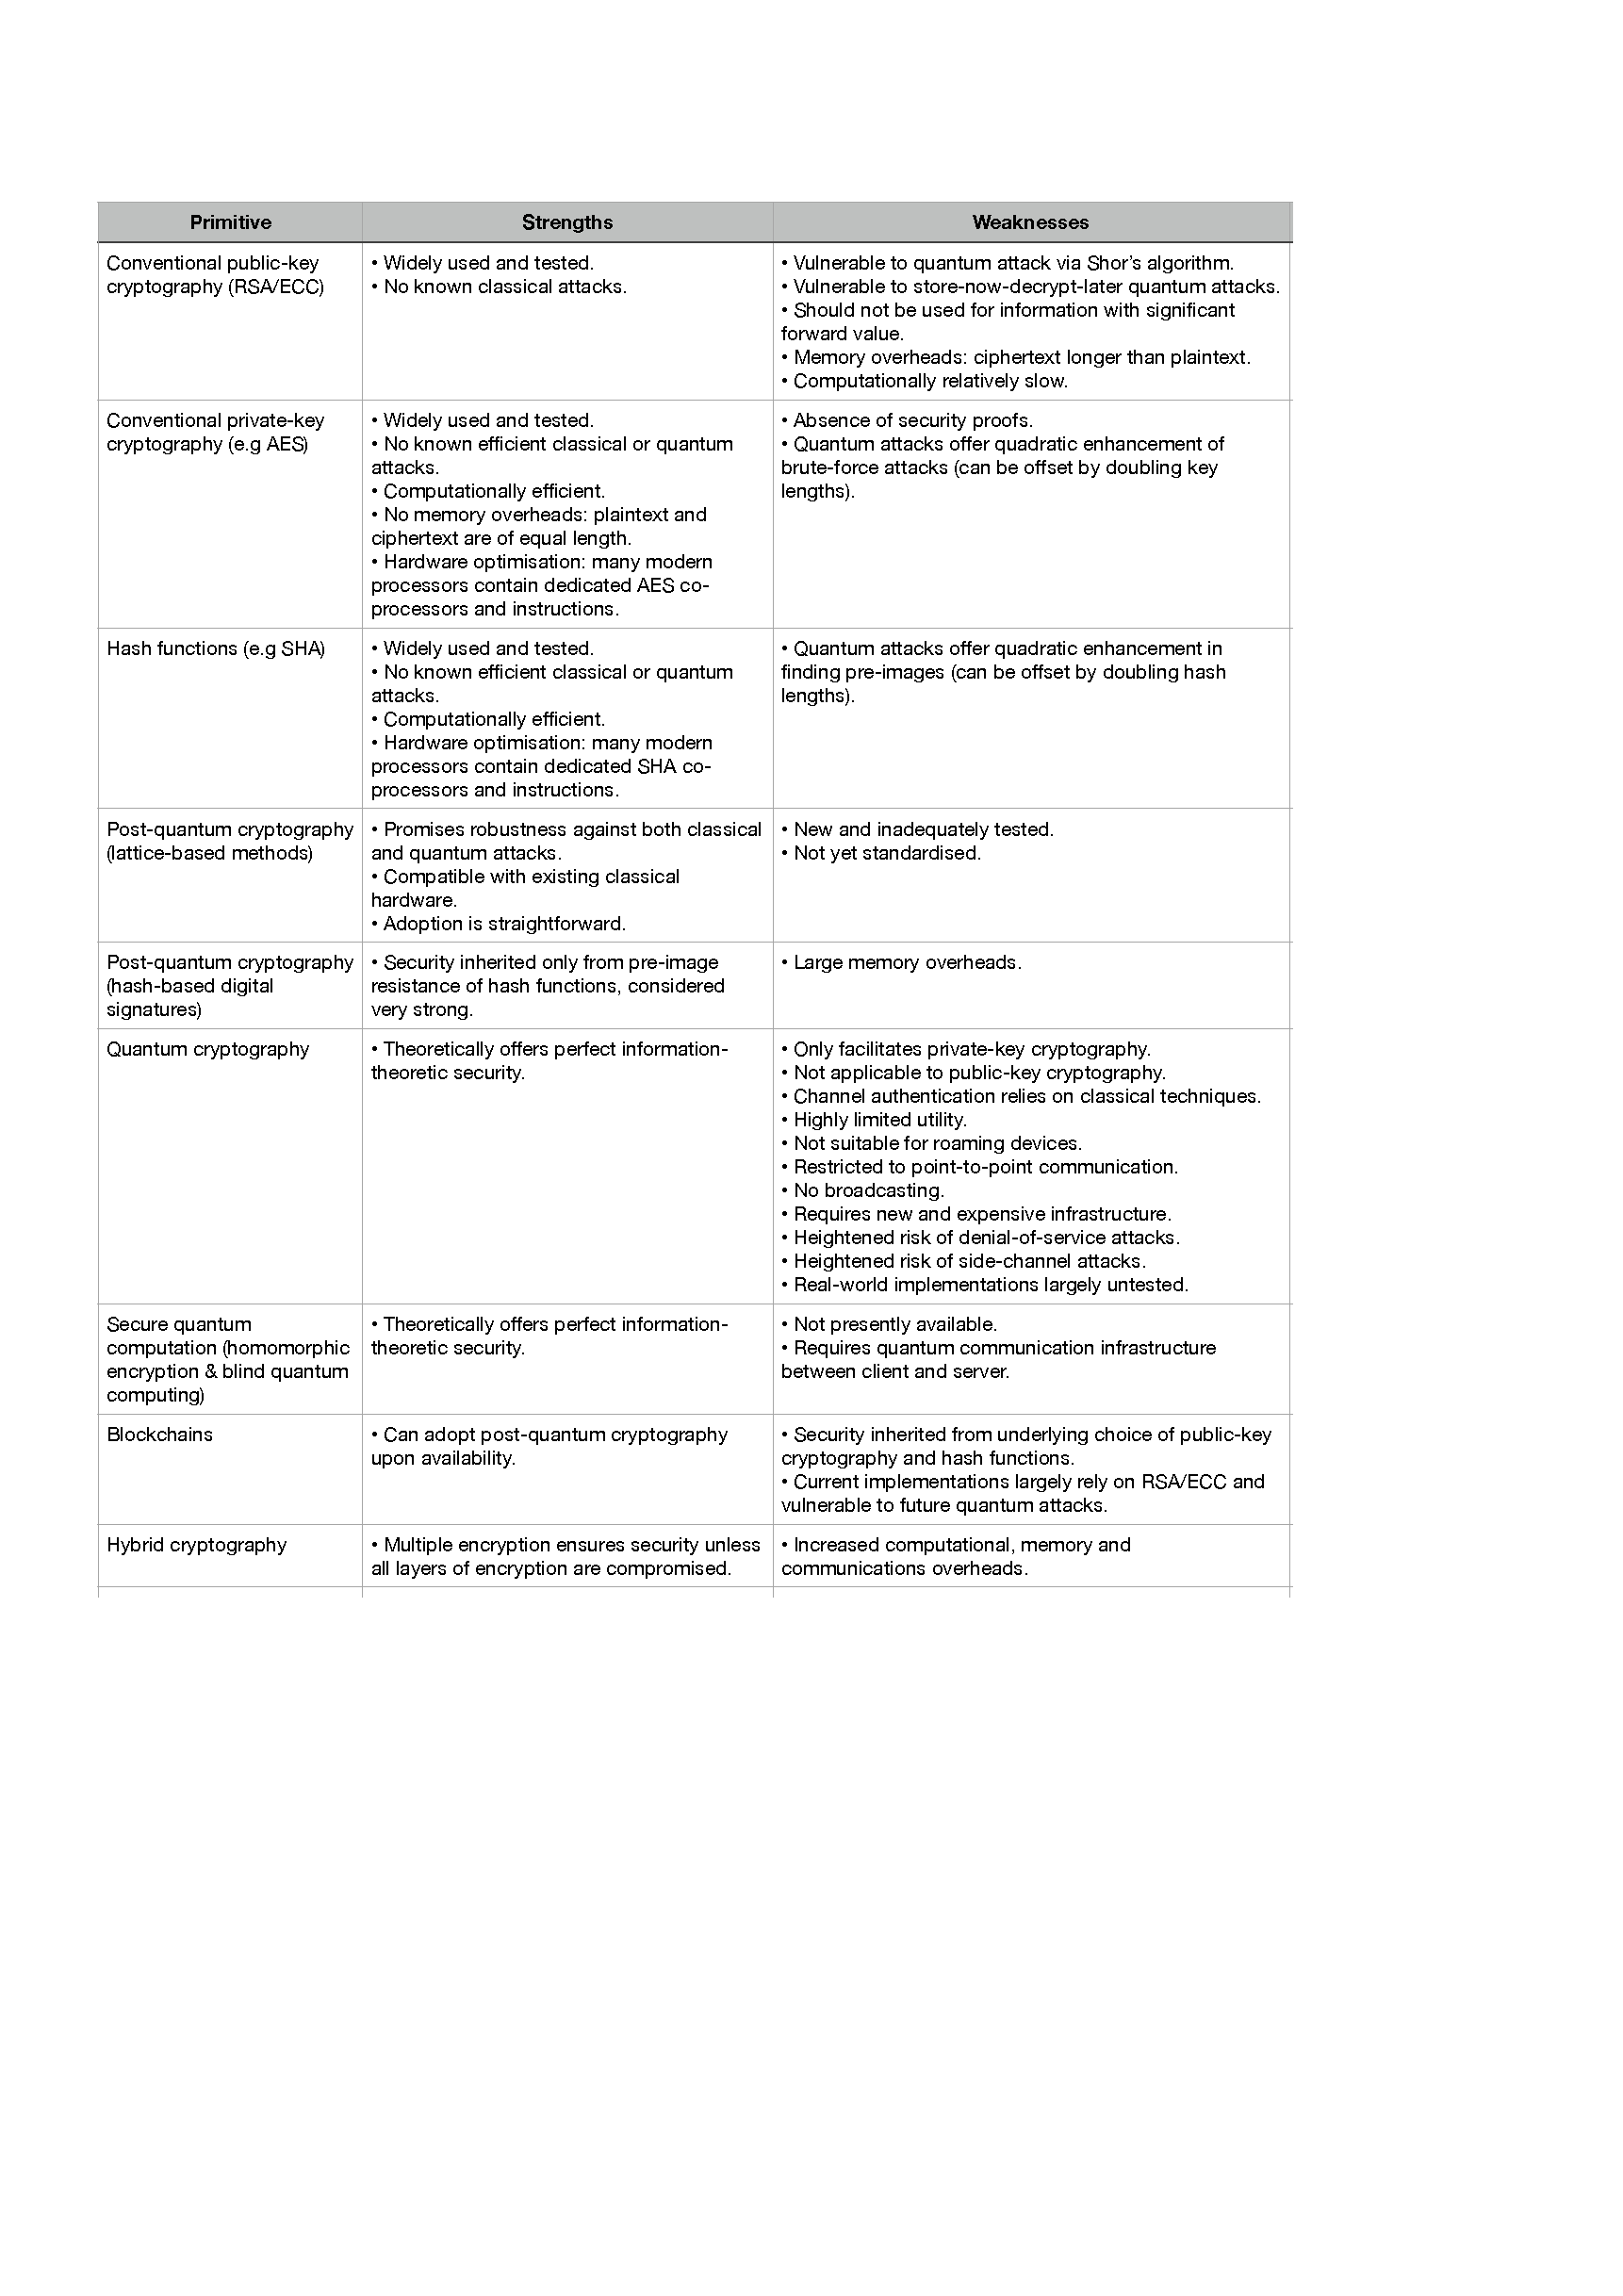
\includegraphics[width=\linewidth]{figures/pros_and_cons}
\caption{Summary of classical and quantum cryptographic primitives and their respective strengths and weaknesses.} \label{fig:pros_and_cons}
\end{figure*}

\subsection{Stored information} \label{stored-information}

While quantum computers of sufficient size to compromise current public key cryptography are likely on the order of a decade or two away, the threats they present are relevant today. It's well known that signals intelligence (SIGINT) agencies around the world, such as the NSA, store encrypted intelligence data that they are presently unable to crack in case some day further down the line they are able to. Since significant amounts of this data will still have strategic or IP relevance in the future, many are no doubt nervous about the prospects of their information being decrypted by adversaries down the line.

It can be taken for granted that nation states are mindful of this when employing encryption protocols today and actively attempt to future-proof their cryptographic protocols against quantum attack vectors or future advancements in cryptanalysis. It is impossible to know what cryptographic advancements have been made by leading SIGINT agencies --- the NSA is purported to be the world's largest employer of mathematicians and needless to say knows far more about cryptography than what is publicly available. Advanced nation states may or may not have developed and employ post-quantum cryptography as part of their cryptographic suites. However what is highly likely is that highly sensitive information is:
\begin{itemize}
	\item Encrypted using keys derived from multiple independent key distribution avenues to minimise the risk of compromised keys being employed.
	\item Multiply encrypted using different encryption algorithms to minimise the risk of unknown vulnerabilities in a given encryption scheme being exploited. PQC would inevitably be a component of such cryptographic suites.
	\item Private keys are derived from multiple independent sources to minimise the likelihood of interception compromising keys.
\end{itemize}

\subsection{Irrelevant information}

While there are troves of data with enormous forward value, to the contrary there are swathes of data of high value today that will be of little or no value tomorrow. Enormous amounts of today's encrypted information will be irrelevant if cracked in the future. For example, when we perform online bank transactions using secure links, once transactions are complete eavesdropping on them is of little value and it isn't possible to manipulate the transaction retrospectively. The issue of \emph{key expiry} is the main point here. If keys are used temporarily for a short period for the sake of some transaction (as opposed to an important communication) and then discarded, this may pose little or no threat.

\subsection{Quantum key distribution}

While QKD offers in principle perfect secrecy of shared bit-strings for use in a one-time-pad or other symmetric cipher, it is far more vulnerable to denial-of-service (Sec.~\ref{denial-of-service-dos-attacks}) and side-channel attacks (Sec.~\ref{side-channel-attacks-qkd}) than classical technology.

Regardless how advanced and mainstream quantum engineering becomes, quantum communications infrastructure will likely always be far more expensive than classical infrastructure. Combined with its more limited use cases this implies quantum networks will be far more sparse than classical ones making them more vulnerable to denial of service attacks.

In the context of military conflict, QKD's vulnerability to denial-of-service is a significant issue, as entities relying on this technology are likely to also be ones of high strategic importance.

QKD will inevitably always be more expensive than classical cryptography, and its use-cases far more limited. Most importantly, QKD only enables private-key cryptography, making it useless for most contemporary applications requiring public-key cryptography. If it is to be used at all, it should be as part of an encryption policy that hybridises it with best-practise classical cryptography, such that the QKD does not act as a single point of failure.

Additionally, quantum information cannot be broadcast in the same way classical information can, rendering it unsuitable for roaming devices on shared networks such as cellular networks.

QKD should be regarded as a technology to compliment rather than replace classical cryptography.

Additionally, it should be noted that secure communications channels additionally require authentication, which reverts back to classical techniques.

Some major Western signals intelligence agencies have released position statements on quantum cryptography. GCHQ, the signals intelligence agency of the United Kingdom \href{https://www.ncsc.gov.uk/whitepaper/quantum-security-technologies}{takes the position},
\begin{quote}
``the NCSC does not endorse the use of QKD for any government or military applications, and cautions against sole reliance on QKD for business-critical networks, especially in Critical National Infrastructure sectors.''
\end{quote}
while the NSA of the United States \href{https://www.nsa.gov/Cybersecurity/Quantum-Key-Distribution-QKD-and-Quantum-Cryptography-QC/
}{takes the similar stance},
\begin{quote}
``NSA views quantum-resistant (or post-quantum) cryptography as a more cost effective and easily maintained solution than quantum key distribution. For all of these reasons, NSA does not support the usage of Quantum Key Distribution or Quantum Cryptography to protect communications in National Security Systems, and does not anticipate certifying or approving any QKD or QC security products for usage by NSS customers unless these limitations are overcome.''
\end{quote}

\subsection{Encrypted computation}

In Secs.~\ref{homomorphic-encryption} \& \ref{blind-quantum-computing} we discussed homomorphic encryption and blind quantum computing, approaches for outsourcing quantum computations such that neither an eavesdropper nor the server performing the computation is able to learn what is being processed.

This brings with it unique strategic considerations in a globalised environment. Since some applications for quantum computing have high strategic or commercial value, enabling adversarial states to opaquely utilise quantum computing infrastructure may pose a strategic threat, one that could be hard to quantify given the secrecy of what is being computed. It would be possible, for example, for an adversarial state to utilise sovereign infrastructure to crack their stored data with high intelligence or intellectual property value.

In some jurisdictions quantum computing is already covered under defence export legislation. It is to be expected that as the field heats up in the coming decades and quantum computers become scalable and capable, so will the regulatory frameworks limiting its use. We might very well see quantum alliances of friendly states who freely share quantum resources, which fracture into a number of discrete strategic quantum alliances.

\subsection{Blockchains} \label{blockchains}

Blockchain based transactions are different however. Since the entire ledger is in the public domain and decentralised --- as opposed to sitting on a private server in a bank vault --- the public ledger could be manipulated if the signature keys of others could be obtained. This could manifest itself via manipulation of the consensus algorithms which sign off on transactions, or by directly compromising individual wallets, both of which are protected using digital signatures. Most major blockchain implementations today rely on signature schemes vulnerable to quantum attack via Shor's algorithms.

\subsubsection{Forward value}

This has major implications for the forward value of blockchains. Based on standard forward value pricing models, if an asset has no future value its discounted present-day value is also zero, and smart contracts aren't very smart if they have been invalidated by the time of maturity \cite{bib:rohdequantcrypto}. For this reason, many blockchains are now under development based on quantum-resistant digital signatures.

\subsubsection{Forks}

\subsection{Caveats} \label{caveats}

It also important to bear in mind that although quantum computers can `efficiently' break RSA/ECC encryption, this doesn't mean they are able to do so spontaneously or cheaply. In fact, running a large scale instance of Shor's algorithm would still take considerable time. This raises two important caveats:
\begin{itemize}
	\item Due to high infrastructural cost compared to classical computing, quantum compute power will be reserved for the highest value applications. Breaking into my personal crypto wallet isn't likely to be one of them, and indeed on a cost benefit analysis probably wouldn't ever be worth it.
	\item Given that quantum computers still take significant time and resources to perform public key code breaking, if the lifespan of keys is below this threshold there isn't likely to be a problem. For example, if blockchains are repeatedly hard-forked and personal wallets given a finite lifetime before they are required to transfer to a new wallet address, the quantum computers won't be able to keep up with the rate of change in signatures. This will create a tit-for-tat situation, as we repeatedly switch our keypairs around, ensuring their lifespan is below threshold.
\end{itemize}